%\section{Anforderungen}
%\textit{In diesem Abschnitt soll die Demoanwendung vorgestellt werden, anhand dessen das Proof-of-Concept erstellt wird. Damit das Proof-of-Concept erstellt werden kann, muss die Demoanwendung die zuvor beschriebenen Probleme aufweisen, hierbei sollen die Probleme möglichst realitätsnah sein und nicht frei erfunden.}

Es wird eine Demoanwendung erstellt, welche die Konzepte anhand der \autoref{anf:1020} umsetzt. Dieser Abschnitt beschäftigt sich mit der Vorstellung der Demoanwendung und der repräsentativen Aufgabe, die diese übernimmt.

In der Motivation wurde ein konkretes Problem eines Kunden der Open Knowledge genannt. Damit die Demoanwendung realistisch eine moderne Webanwendung darstellt, wird sie in Grundzügen den Aufbau der Webanwendung des Direktversicherers nachahmen. Bei der Webanwendung handelt es sich um einen Wizard, also einer Sequenz von aufeinanderfolgenden Dialogseiten bei dem der Nutzer Daten eingeben soll. Bei der Webanwendung handelt es sich um eine clientbasierte Angular-SPA. Die Webanwendung validiert einzelne Felder gegen Partnersysteme (bspw. beim Adressfeld). Am Ende des Wizards werden die gesamten Daten an ein weiteres Partnersystem übermittelt, welches darauf basierend eine Berechnung durchführt und das Ergebnis dann an die Webanwendung sendet.

Es wurde sich dafür entschieden, dass die Webanwendung eine Bestellfunktionalität eines Obst-Webshops darstellen soll. Der Warenkorb hierfür wird anfangs dynamisch generiert und dies soll so simulieren, dass eine andere Komponente diesen erstellt hat. Der Nutzer soll seine Rechnungs- und Lieferdaten eingeben und am Ende die Bestellung ausführen können. Um das gewünschte Verhalten der Demoanwendung zu definieren, wird es im folgenden Abschnitt festgelegt.

\subsection{Verhaltensdefinition}

Mit den beiden Stakeholdern, also Christian Wansart und Stephan Müller, die beide am Projekt für den Kunden involviert sind, wurde diese Verhaltensdefinition erstellt. Diesen Ansatz der Definition der Software anhand des Verhaltens nennt man Behavior-Driven Development (BDD). BDD wurde 2006 erstmals von Dan North benannt und definiert \cite{IntroducingBDD}. Bei BDD werden User-Stories aus der Sicht eines äußerlichen Betrachters entworfen und geschrieben. Dabei umfassen die User-Stories Beispiele, wie sich die Anwendung in diesen Szenarien verhalten soll.

Um die BDD-Definition festzuhalten wurde sie in der gängigen Gherkin-Syntax \cite{Gherkin} geschrieben. Die Syntax ist natürlich zu lesen, folgend werden alle gewünschten Features der Demoanwendung in der Gherkin-Syntax aufgelistet.

\lstinputlisting[
  language = gherkin,
   caption = Demoanwendung: Gherkin Definition zum Feature \enquote{Warenkorb},
captionpos = b,
     label = lst:demoanwendung-gherkin-warenkorb
]{content/04_erstellung-poc/warenkorb-gherkin/1-warenkorb.feature}

\lstinputlisting[
  language = gherkin,
   caption = Demoanwendung: Gherkin Definition zum Feature \enquote{Rechnungsadresse},
captionpos = b,
     label = lst:demoanwendung-gherkin-rechnungsadresse
]{content/04_erstellung-poc/warenkorb-gherkin/2-rechnungsadresse.feature}

\lstinputlisting[
  language = gherkin,
   caption = Demoanwendung: Gherkin Definition zum Feature \enquote{Lieferadresse},
captionpos = b,
     label = lst:demoanwendung-gherkin-lieferadresse
]{content/04_erstellung-poc/warenkorb-gherkin/3-lieferadresse.feature}

\lstinputlisting[
  language = gherkin,
   caption = Demoanwendung: Gherkin Definition zum Feature \enquote{Zahlungsdaten},
captionpos = b,
     label = lst:demoanwendung-gherkin-zahlungsdaten
]{content/04_erstellung-poc/warenkorb-gherkin/4-zahlungsdaten.feature}

\lstinputlisting[
  language = gherkin,
   caption = Demoanwendung: Gherkin Definition zum Feature \enquote{Bestellung abschließen},
captionpos = b,
     label = lst:demoanwendung-gherkin-bestellung_abschließen
]{content/04_erstellung-poc/warenkorb-gherkin/5-bestellung_abschließen.feature}

Neben dem eigentlichen User-Interface soll auch ein Backend Teil der Demoanwendung sein. Hierfür wurde auf Basis der Verhaltensdefinition eine Architektur entworfen, die im folgenden Abschnitt näher beschrieben wird.

\subsection{Backend}

Das Backend wurde als Microservice-Architektur konzipiert und wurde ebenso wie die Webanwendung auch an das Projekt des Open Knowledge Kunden angelehnt. In \autoref{fig:demoanwendung_deployment} lässt sich die konzipierte und umgesetzte Architektur betrachten, hierbei stellen Pods einzelne Containersysteme dar. Diese Architektur wurde mit den Stakeholdern zusammen konzipiert und ähnelt dem des Direktversicherers.

Für das Frontend ist die einzig anzusprechende Schnittstelle das \enquote{backend4frontend}, welches die Kommunikation zu Partnersystemen ermöglicht sowie die Sicherheits- und Validitätsaspekte überprüft. Die weiteren Dienste \enquote{Bestellungen}, \enquote{Übersetzungen}, \enquote{Addressvalidierung} und \enquote{Warenkorb} übernehmen die jeweilige Funktion, die ihr Name beschreibt. Der Dienst \enquote{Bestellungen} ist das Partnersystem, welches beim Fertigstellen des Wizards aufgerufen wird und es führt dabei weitere Datenabfragen und Validitätsüberprüfungen mit Partnerdiensten durch.

Mit dieser recht komplexen Architektur einer Demoanwendung wurde versucht, eine möglichst realitätsnahe Repräsentation zu erstellen. Speziell wird bei einer solchen Architektur der Nutzen von Tracing deutlicher, nämlich um z. B. die Zusammenhänge zwischen den Diensten nachvollziehen zu können. Dies wird beim Einsatz und der Vorstellung der Lösung näher betrachtet.

\begin{figure}[H]
	\centering
	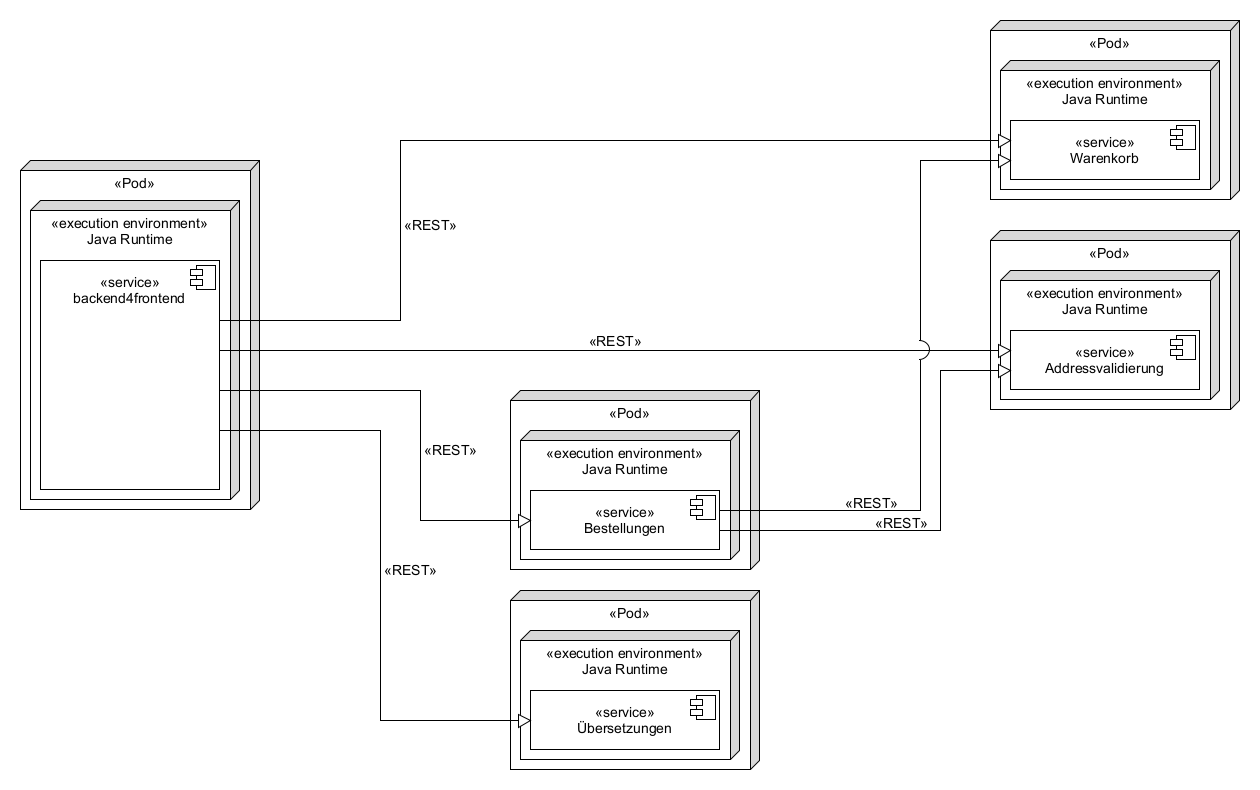
\includegraphics[width=1.00\linewidth]{img/04_erstellung-poc/demoanwendung_deployment.png}
	\caption{Demoanwendung: Deployment-Diagramm, Quelle: Eigene Darstellung}
	\label{fig:demoanwendung_deployment}
\end{figure}

\newpage

\subsection{Frontend}

Wie beim Kunden wurde ein Wizard auf Basis von Angular erstellt, welcher mehrere aufeinander folgende Formulare in derselben SPA enthält. In den folgenden Abschnitten wird das Frontend anhand eines Beispieldurchlaufs durch die einzelnen Seiten vorgestellt.

\subsubsection{Warenkorb}

\autoref{fig:demoanwendung_vorstellung_01-warenkorb} zeigt die Startseite, die der Nutzer sieht, wenn er die Demoanwendung aufruft. Hierbei wird simuliert, dass der Nutzer zuvor in einem Online-Obsthandel einige Produkte ausgewählt hat und sich nun auf der Ansichtsseite des Warenkorbs befindet. Hier kann der Nutzer seine Auswahl prüfen und bei Zufriedenheit kann er den Bestellvorgang starten. Die hier angezeigten Daten werden vom Warenkorbdienst abgerufen, über die Angabe eines zuvor zufällig generierten Warenkorb-Identifiers. Die Warenkorbdaten werden zudem mit Übersetzungsdaten vom Übersetzungsdienst angereichert, denn in den Warenkorbdaten stehen lediglich Übersetzungsschlüssel wie \texttt{item.peach}, die dann auf den tatsächlichen Übersetzungswert abgebildet werden also \texttt{Pfirsich}. Beim Starten des Bestellvorgangs wird keine Serverabruf durchgeführt, sondern in der SPA ein Seitenwechsel vorgenommen.

\begin{figure}[H]
	\centering
	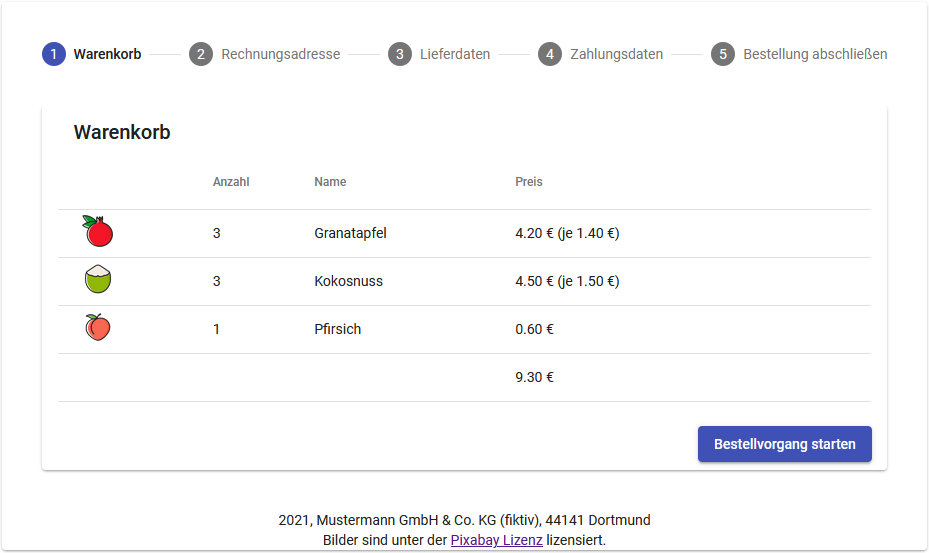
\includegraphics[width=1.00\linewidth]{img/04_erstellung-poc/demoanwendung_vorstellung_01-warenkorb.png}
	\caption{Demoanwendung: Startseite \enquote{Warenkorb}}
	\label{fig:demoanwendung_vorstellung_01-warenkorb}
\end{figure}

\subsubsection{Rechnungsadresse}

Startet der Nutzer den Bestellvorgang, so landet er zunächst auf der Eingabemaske zur Rechnungsadresse (vgl. \autoref{fig:demoanwendung_vorstellung_02-rechnungsadresse}). Hier wird er gebeten rechnungsrelevante Informationen anzugeben, u. A. seine Adresse. Er kann jedoch auch auf die vorherige Seite zurückspringen.

Beim Absenden des Formulars wird zunächst die Validität der Eingabefelder überprüft, bspw. ob die PLZ aus 5 Zahlen besteht, und anschließend wird die Adresse dem Adressvalidierungsdienst zur Prüfung übergeben. Schlägt eine Validierung fehl, so wird dies entweder direkt am verursachenden Textfeld angezeigt oder in einer allgemeinen Fehlermeldung im unteren Bereich der Eingabemaske ausgegeben.

Sind beide Prüfungen jedoch erfolgreich, so wird ein Seitenwechsel in der SPA durchgeführt. Neben der Adressüberprüfung wird kein zusätzlicher Serveraufruf durchgeführt, die eingegeben Daten werden jedoch intern einer übergreifenden Komponente übergeben.

\begin{figure}[H]
	\centering
	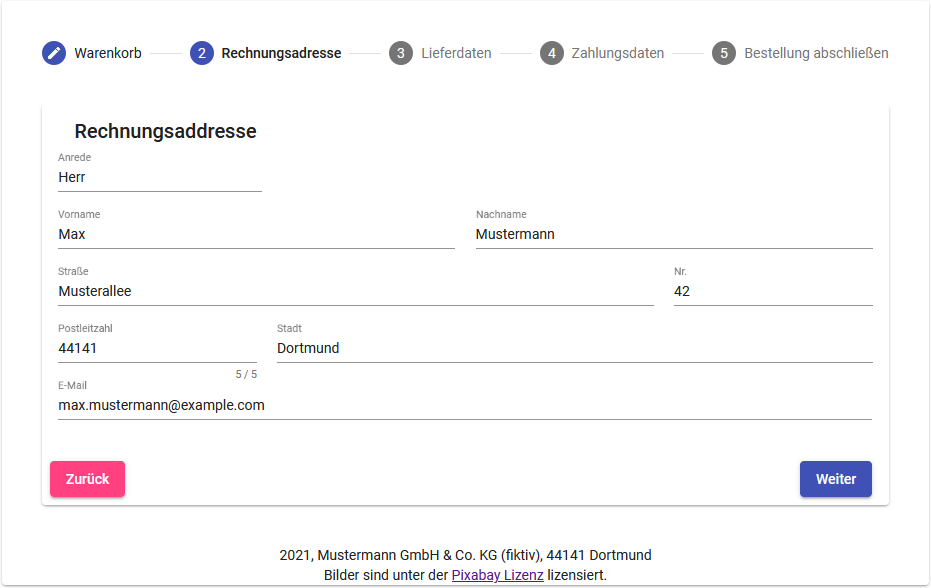
\includegraphics[width=1.00\linewidth]{img/04_erstellung-poc/demoanwendung_vorstellung_02-rechnungsadresse.png}
	\caption{Demoanwendung: Seite \enquote{Rechnungsadresse}}
	\label{fig:demoanwendung_vorstellung_02-rechnungsadresse}
\end{figure}

\newpage

\subsubsection{Lieferdaten}

Nach einer erfolgreichen Eingabe der Rechnungsadresse, wird der Nutzer nun gebeten seine Daten einzugeben, wo die Produkte hin geliefert werden sollen. Hierzu kann er entweder die relevanten Daten aus der Rechnungsübernehmen lassen (Standardfall) oder er gibt alternativ abweichende Lieferdaten an, wie in \autoref{fig:demoanwendung_vorstellung_03-lieferdaten} zu sehen ist. Wie zuvor kann der Nutzer auch auf das vorherige Formular zurückspringen.

Bei der Angabe von abweichenden Lieferdaten werden, wie beim Formular der Rechnungsadresse, zunächst die Eingabefelder überprüft und bei Fehlschlag visuell dem Nutzer darüber berichtet. Anders als bei der Rechnungsadresse wird jedoch nicht die Adressvalidierungsdienst befragt, dies wird in \label{sec:invalid-address-is-valid} aufgefasst und erläutert.

Sind keine abweichenden Lieferdaten erwünscht oder die Validierung der Eingaben erfolgt, wird beim Klick auf \enquote{Weiter} ein Seitenwechsel in der SPA durchgeführt. Auch hier erfolgt kein Serveraufruf, jedoch werden die Daten an die übergreifende Komponente innerhalb der Webanwendung weitergereicht.

\begin{figure}[H]
	\centering
	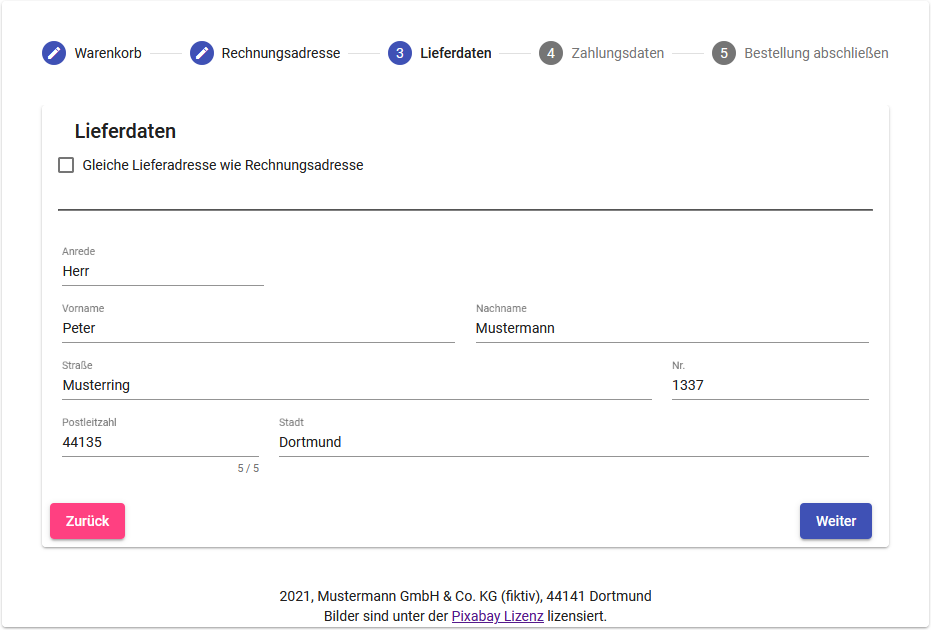
\includegraphics[width=1.00\linewidth]{img/04_erstellung-poc/demoanwendung_vorstellung_03-lieferdaten.png}
	\caption{Demoanwendung: Seite \enquote{Lieferdaten}}
	\label{fig:demoanwendung_vorstellung_03-lieferdaten}
\end{figure}

\subsubsection{Zahlungsdaten}

Anschließend der Eingabe der Lieferdaten wird der Nutzer nun gebeten seine Zahlungsinformationen einzugeben. Hierbei kann der Nutzer zwischen 4 Zahlungsarten auswählen: per Rechnung, Lastschrift, PayPal oder Kreditkarte. Wie bei den anderen Formularen kann der Nutzer auf das vorhergehende Formular über den Button \enquote{Zurück} wechseln.

Bei Auswahl der Rechnungsart \enquote{Rechnung} muss der Nutzer keine weiteren Daten eingeben. Hingegen sind bei anderen Rechnungsarten weitere Daten einzugeben, wie z. B. der in der \autoref{fig:demoanwendung_vorstellung_04-zahlungsdaten} zu betrachteten Rechnungsart \enquote{Lastschrift}, hier muss der Kontoinhaber und die IBAN angegeben werden. Bei PayPal muss die PayPal-E-Mail werden und bei der Auswahl der Kreditkarte müssen die Kreditkarteninformationen Karteninhaber, Kartennummer, CVC sowie das Ablaufdatum angegeben werden. Die jeweilig einzugebenden Daten werden clientseitig validiert, ähnlich wie bei den vorherigen Formularen.

Ist eine Rechnungsart ausgewählt und die einzugebenden Daten valide ausgefüllt, so führt ein Absenden des Formulars zu einem Seitenwechsel auf die Seite zum Abschließen der Bestellung. Es wird keine zusätzliche Serverinteraktion durchgeführt, die Daten werden jedoch erneut an die übergreifende Komponenten übergeben.

\begin{figure}[H]
	\centering
	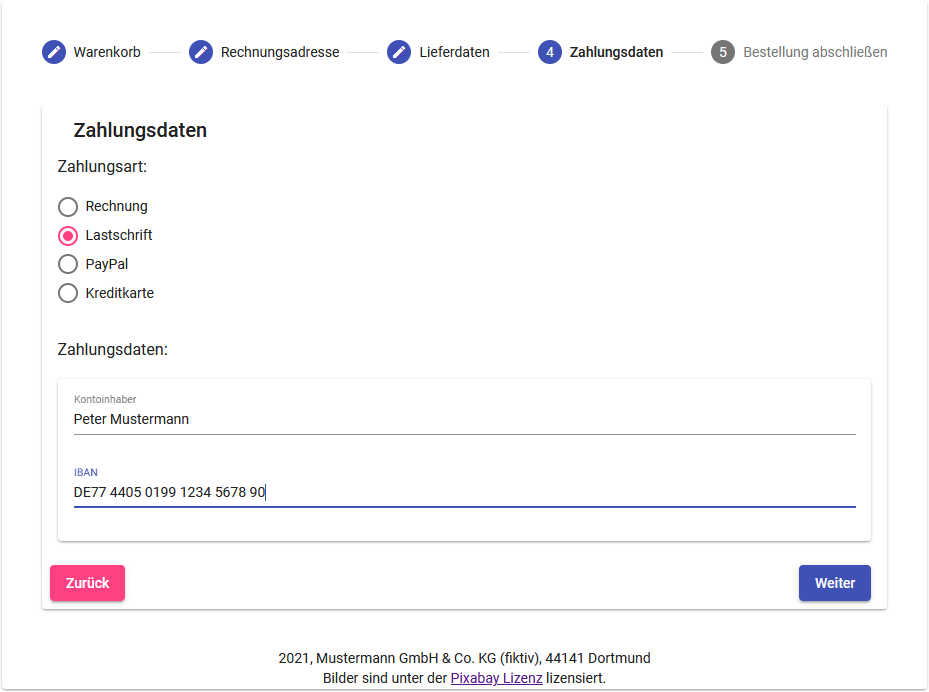
\includegraphics[width=0.90\linewidth]{img/04_erstellung-poc/demoanwendung_vorstellung_04-zahlungsdaten.png}
	\caption{Demoanwendung: Seite \enquote{Zahlungsdaten}}
	\label{fig:demoanwendung_vorstellung_04-zahlungsdaten}
\end{figure}

\subsubsection{Bestellübersicht}

Da der Nutzer nun alle notwendigen Daten zur Bestellung eingegeben hat, wird auf dieser Seite ihm eine Übersicht dieser Eingaben präsentiert, wie in \autoref{fig:demoanwendung_vorstellung_05-bestelluebersicht} zu sehen ist. Wie bei allen Formularen gibt es auch hier die Option für den Nutzer zu einem vorherigen Formular zurückzuspringen und Anpassungen vorzunehmen.

In der Bestellübersicht werden explizit der ausgewählte Warenkorb, die eingegebenen Rechnungs- und Lieferadresse sowie die gewählte Zahlungsart dargestellt. Der Warenkorb wird hierbei analog zur Warenkorbseite vom Warenkorbdienst abgefragt und nicht clientseitig gespeichert. Die anderen Daten sind nur clientseitig gespeichert und werden über eine übergreifende Komponente bereitgestellt. Weitere Eingaben sind auf dieser Seite vom Nutzer aber nicht gefordert, sie dient hauptsächlich der visuellen Überprüfung für den Nutzer bevor er die Bestellung kostenpflichtig durchführt.

Sendet der Nutzer die Bestellung ab, werden die zuvor eingegeben Daten und der Identifier des Warenkorbs an den Bestelldienst übergeben. Dieser überprüft beide Adresseingaben gegen den Adressvalidierungsdienst, ruft den Warenkorb vom Warenkorbdienst ab und errechnet auf dieser Datenbasis den Bestellbeleg. Der Bestellbeleg wird dem Frontend in der Antwort übergeben und dies führt zu einem Seitenwechsel.

\begin{figure}[H]
	\centering
	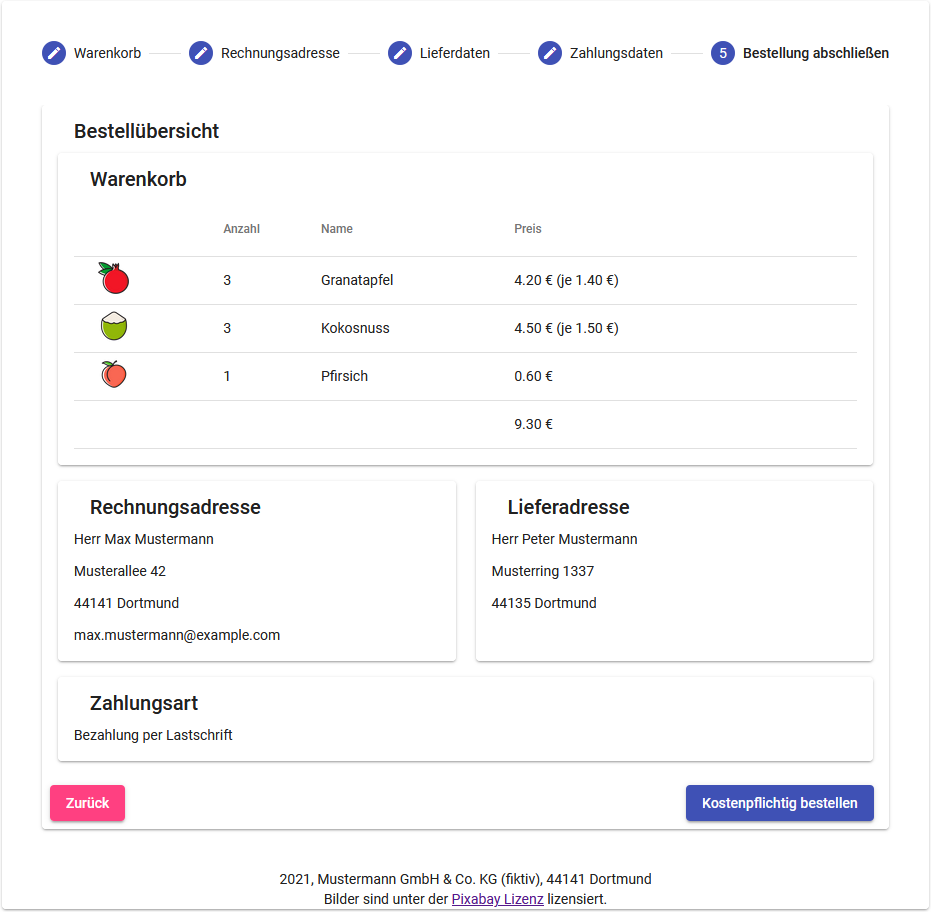
\includegraphics[width=0.65\linewidth]{img/04_erstellung-poc/demoanwendung_vorstellung_05-bestelluebersicht.png}
	\caption{Demoanwendung: Seite \enquote{Bestellübersicht}}
	\label{fig:demoanwendung_vorstellung_05-bestelluebersicht}
\end{figure}

\subsubsection{Bestellbestätigung}

Über die erfolgreiche Bestellung leitet die SPA automatisch auf diese Seite weiter. Hier werden die Daten der Bestellbestätigung dem Nutzer visuell präsentiert (vgl. \autoref{fig:demoanwendung_vorstellung_06-bestellbestaetigung}). Bei den angezeigten Daten handelt es sich nicht um die zuvor gespeicherten, sondern ausschließlich um die vom Bestelldienst übermittelten Daten.

Auf dieser Seite kann der Nutzer nun nur noch auf den Button \enquote{Zum Shop} klicken und gelangt erneut zur Startseite, jedoch mit einem neuen Warenkorb.

\begin{figure}[H]
	\centering
	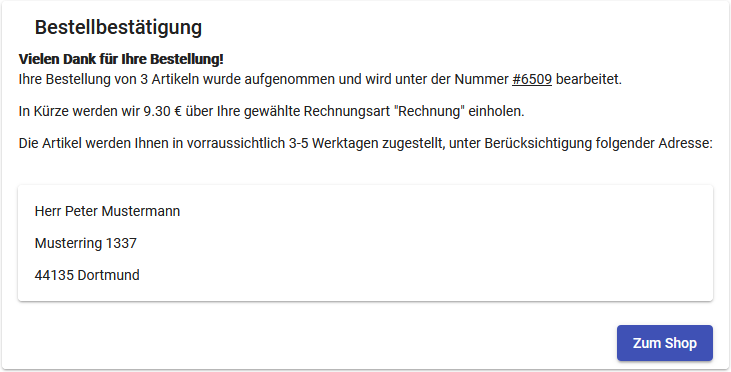
\includegraphics[width=0.75\linewidth]{img/04_erstellung-poc/demoanwendung_vorstellung_06-bestellbestaetigung.png}
	\caption{Demoanwendung: Finale Seite \enquote{Bestellbestätigung}}
	\label{fig:demoanwendung_vorstellung_06-bestellbestaetigung}
\end{figure}

Wie in \autoref{anf:1020} definiert wurden in das Frontend einige Fehler eingebaut, damit diese, mit der zu erstellenden Lösung, aufgedeckt werden können. Diese Fehler werden nachfolgend näher betrachtet.

\subsection{Fehlerszenarien}
\label{subsec:fehlerszenarien}

Wie zuvor erwähnt und in \autoref{anf:1020} gewünscht, besitzt die Demoanwendung einige simulierte Fehler. Diese Fehler wurden in Zusammenarbeit mit den Stakeholdern konzipiert. Bei der Konzeption wurde versucht möglichst realitätsnahe oder sogar tatsächlich beim Kunden aufgetretene Probleme einzubauen.

Diese Fehler gehören unterschiedlichen Problemgruppen an, sie reichen von unerwünscht strenger Validierung, über Konfigurationsfehlern bis hin zu ineffizienter Datenverarbeitung. Sie werden folgen in Fehlerszenarien beschrieben, aus der Sicht eines Projektteams, welches diese Szenarien berichtet bekommen oder selbst notiert hat.

\subsubsection{\enquote{Keine Übersetzungen}}

\begin{wrapfigure}[6]{r}{0.33\textwidth}
\centering
\vspace{-\baselineskip}
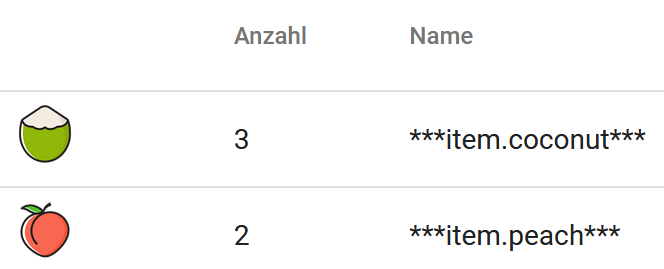
\includegraphics[width=\linewidth]{img/04_erstellung-poc/demoanwendung_fehlerszenario-uebersetzungen}
\caption{Fehlende Texte}
\label{fig:demoanwendung_fehlerszenario-uebersetzungen}
\end{wrapfigure}

- Problem: Nutzer berichten, dass manchmal die Webanwendung beim Start keine Artikeltexte anzeigt (vgl \autoref{fig:demoanwendung_fehlerszenario-uebersetzungen}).

- Ursache: Die Pods, die den Übersetzungsdienst enthalten werden repliziert bereitgestellt. Einer der Pods hat eine defekte Konfiguration, weswegen er keine Übersetzungen der Artikel enthält. Wird zu diesem Pod verbunden, tritt das Fehlverhalten auf. Dies ist eine Nachstellung eines tatsächlichen Problems beim Kunden.

\subsubsection{\enquote{Gültige Straßen sind ungültig}}

- Problem: Nutzer berichten, dass Ihr Straßenname nicht eingeben werden kann. Beispielsweise führt die Eingabe \enquote{Ährenweg} zu einem Fehler.

- Ursache: Der Adressvalidierungsdienst validiert Straßen mit dem Regular-Expression \texttt{[a-zA-Z\textbackslash,\textbackslash-\textbackslash ]+}, welches keine gängigen Sonderzeichen (ä ,ö ,ü, ß) erlaubt.

\subsubsection{\enquote{Gültige Hausnummern sind ungültig}}

- Problem: Nutzer berichten, dass Hausnummern, die nicht nur aus Zahlen bestehen, zum Fehler führen.

- Ursache: Der Adressvalidierungsdienst validiert Hausnummern als Zahl und schlägt im o. g. Fall in der Konvertierung fehl.

\subsubsection{\enquote{Gültige Städte sind ungültig}}

- Problem: Nutzer aus Gießen berichten, dass Sie das Formular zur Rechnungsadresse nicht ausfüllen können

- Ursache: Der Adressvalidierungsdienst meldet die Stadt \enquote{Gießen} als ungültig, weil sie nicht in der lokalen Tabelle vorhanden ist.

\subsubsection{\enquote{Ungültige Adressen sind gültig}}
\label{sec:invalid-address-is-valid}

- Problem: Nutzer können in den Lieferdaten ungültige Eingaben tätigen und absenden, bei der Bestellaufgabe kommt es zu einem Fehler.

- Ursache: Das Frontend überprüft lediglich die Rechnungsadresse, aber nicht die Lieferadresse

\subsubsection{\enquote{Vor- und Nachnamen werden abgeschnitten}}

- Problem: Nutzer berichten, dass in der Bestellbestätigung Ihre Vor- und Nachnamen abgeschnitten dargestellt werden.

- Ursache: Der Bestelldienst begrenzt den Vor- sowie den Nachnamen auf 20 Zeichen, das Frontend begrenzt dies jedoch nicht.

\subsubsection{\enquote{Falsche Zahlungsart}}

- Problem: Nutzer berichten, dass in der Bestellbestätigung die falsche Zahlungsart angezeigt wird. In der Bestellübersicht wurde jedoch die korrekte Zahlungsart angezeigt.

- Ursache: Das Frontend sendet alle Formulardaten jeder Rechnungsart an den Dienst \enquote{Bestellungen}. Dieser nimmt aber an, dass alle nicht ausgewählten Rechnungsarten statt Formulardaten nur \texttt{null} enthalten.

\subsubsection{\enquote{Lange Verarbeitung}}

- Problem: Beim Absenden des Formulars auf der Seite \enquote{Warenkorb} kommt es zu einer unerwünschten Wartezeit (von min. 6-10s).

- Ursache: Dies ist eine simulierte Wartezeit im Frontend je nach Anzahl der Positionen (2s pro Position), um eine ineffiziente Verarbeitung nachzuahmen.

\subsection{Repräsentation}

Eine wichtige Eigenschaft der Demoanwendung sollte sein, dass sie repräsentativ für die Webanwendung des Kunden ist und im Allgemeineren auch für moderne Webanwendungen ist. Durch den groben Aufbau der Demoanwendung, also einer zustandsreichen und zu großen Teilen clientbasierten SPA, stellt die Demoanwendung eine moderne Webanwendung dar. Auch die Verwendung von Angular ist repräsentativ, denn Angular ist eines der meist verwendeten Frontend-Frameworks \cite{TheStateOfJavaScript2020}.

Das Backend ist in dem Sinne repräsentativ, dass es auf keiner stark vereinfachten Infrastruktur basiert, sondern gewollt an die Situation des Open Knowledge Kunden abbildet. Des Weiteren stellt die gewählte Architektur einen modernen Ansatz dar, denn die Architektur ist Microservice-orientiert \cite{MicroserviceArchitecture}.

Dennoch ist anzumerken, dass die Demoanwendung nur ein Modell einer tatsächlichen Webanwendung darstellt. Wie jedes Modell können nicht alle Gegebenheiten des zu modellierenden Sachverhalts nachgestellt werden. Jedoch ist durch den allgemein gehaltenen Anwendungsfall und die moderne Umsetzung eine Übertragbarkeit zu ähnlichen Projekten durchaus vorhanden.

Nun da die Demoanwendung beschrieben ist, wird das Konzept erstellt, welches letztendlich auf die Demoanwendung anzuwenden ist. Das Konzept selber ist jedoch losgelöst von der Demoanwendung zu verstehen.